%% Requires compilation with XeLaTeX or LuaLaTeX
\documentclass[10pt,xcolor={table,dvipsnames},t]{beamer}
\usetheme{UCBerkeley}
\usepackage[utf8]{inputenc}
\usepackage{tikz}
\title[Your Short Title]{Solving 2D geometric problems using matrices}
\subtitle{Your subtitle (if there's one)}
\author{Sivani\\Varsha}
\institute{Electrical}
\date{Date of Presentation:14 Feb,2019}

\begin{document}

\begin{frame}
  \titlepage
\end{frame}

% Uncomment these lines for an automatically generated outline.
%\begin{frame}{Outline}
%  \tableofcontents
%\end{frame}

\section{Introduction}

\begin{frame}{Geometric Problem}

\begin{itemize}
  \item A circle whose radius is 3 touches externally the circle C at point (2,2).The circle C is x^2+y^2+4x-2y-4=0.
  
\end{itemize}

\begin{block}{}
Then find the length of intercept made by that Circle on X-axis.
\end{block}

\end{frame}

\section{Some \LaTeX{} Examples}

\subsection{Mathematics}

\begin{frame}{Matrix Transformation}
\begin{equation}
x^Tx+
\begin{bmatrix}
-2 &&
 4
\end{bmatrix}
x -4=0
\end{equation}
intersects the circle at point
\begin{bmatrix}
2 \\
2

\end{bmatrix}
Then,find intercept made by circle on x-axis by using matrices.

\end{frame}

\subsection{Tables and Figures}

\smallframetitle

\begin{frame}{Solution using matrices}

Given point B =
\begin{bmatrix}
2 \\ 
2
\end{bmatrix}
is midpoint of A =
\begin{bmatrix}
x \\
y
\end{bmatrix}
and C = 
\begin{bmatrix}
-1 \\
2
\end{bmatrix}

Where A,C are centers of circles and B is point of intersection of those circles. 
So,from above conditions we get A =
\begin{bmatrix}
5 \\
2

\end{bmatrix}
Given radius of circle is 3,the equation of circle in matrix form is
C' = 
\begin{equation}
x^Tx+
\begin{bmatrix}
-10 &&
-4
\end{bmatrix}
x +20= 0

\end{equation}

\end{frame}

\begin{frame}
\frametitle{Intercept on x-axis}
To find intercept on x-axis ,y co-ordinate should be zero.so,we get a quadratic equation,
\begin{equation}
    x^2-10x+20 = 0
\end{equation}
The roots of above equation are
D = 
\begin{bmatrix}
7.236 \\
2.764
\end{bmatrix}
.Take a matrix 
M = 
\begin{bmatrix}
1 &&
-1
\end{bmatrix}
Then,distance d is
\begin{equation}
d = DM

\end{equation}
Then,by matrix multiplication,distance
\begin{equation}
    d = 4.472
\end{equation}
\end{frame}

\begin{frame}
\begin{figure}
\frametitle{Figure of solution}
\begin{tikzpicture}
\draw (5,2) circle (3cm);
\draw (-1,2) circle(3cm);
\draw(2,2) circle(2pt)  node [right] {$(2,2)$};;
\fill (2,2) circle[radius = 3pt]


\end{tikzpicture}
\end{figure}
\end{frame}

\normalframetitle

\begin{frame}
\frametitle{Uploaded photo from python code}

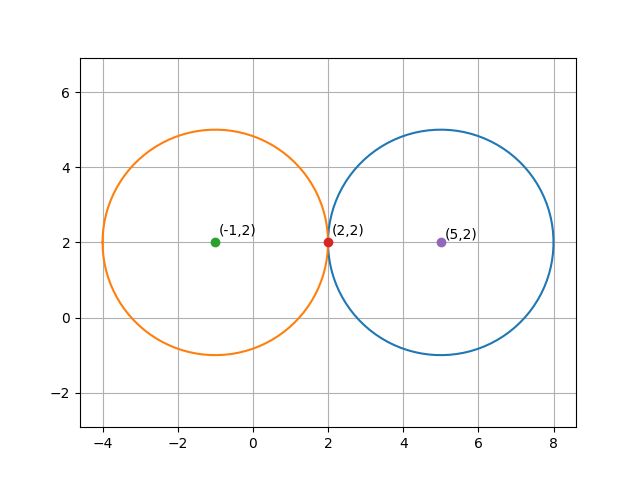
\includegraphics[width=.90\textwidth,height=.7\textheight]{circle.png}

\end{frame}


\end{document}
